\documentclass[conference]{IEEEtran}
\IEEEoverridecommandlockouts
% The preceding line is only needed to identify funding in the first footnote. If that is unneeded, please comment it out.
\usepackage{cite}
\usepackage{amsmath,amssymb,amsfonts}
\usepackage{algorithmic}
\usepackage{graphicx}
\usepackage{textcomp}
\usepackage{caption}
\captionsetup[table]{labelfont=normalfont,textfont=normalfont}
\usepackage{xcolor}
\usepackage{hyperref}
\usepackage{float}
\usepackage{tikz} 
\usepackage{booktabs}
\usetikzlibrary{positioning, arrows.meta, shapes.geometric}

\def\BibTeX{{\rm B\kern-.05em{\sc i\kern-.025em b}\kern-.08em
		T\kern-.1667em\lower.7ex\hbox{E}\kern-.125emX}}
\begin{document}

\title{Controle de sala climatizada\\
	{\footnotesize \textsuperscript{Sistemas em Tempo Real}}
}

\author{\IEEEauthorblockN{1\textsuperscript{st} Davi Sales de Sousa}
	\IEEEauthorblockA{\textit{180015401} \\
		\textit{Engenharia Mecatrônica - UnB}\\
		Brasília, Brasil \\
		davi.sales@aluno.unb.br}
	\and
	\IEEEauthorblockN{2\textsuperscript{nd} Giovanna Nogueira Freire}
	\IEEEauthorblockA{\textit{200018710} \\
		\textit{Engenharia Mecatrônica - UnB}\\
		Brasília, Brasil \\
		giovanna.freire@aluno.unb.br}
	\and
	\IEEEauthorblockN{3\textsuperscript{rd} Luiz Felipe Ducat}
	\IEEEauthorblockA{\textit{231035400} \\
		\textit{Ciência da Computação - UnB}\\
		Brasília, Brasil \\
		luiz.ducat@aluno.unb.br}
	\and
	\IEEEauthorblockN{4\textsuperscript{th} Pedro Dantas Freitas}
	\IEEEauthorblockA{\textit{200026011} \\
		\textit{Engenharia Mecatrônica - UnB}\\
		Brasília, Brasil \\
		freitas.pedro@aluno.unb.br}
}
\maketitle

\begin{abstract}
	
	Este trabalho o desenvolvimento da solução para o problema de regulação do clima ambiente baseada nos princípios de sistemas de tempo real. A solução implementada é composta por um sistema com um sensor de umidade do ar e temperatura e dois atuadores: um umidificador de ar, ventilador 12V, visor LCD para verificar status, botões para interação com o sistema e um arduino uno para controle e execução das tarefas. Tal implementação é feita em escala reduzida por praticidade e disponibilidade de materiais, entretando, os conceitos de modelagem utilizados podem ser extrapolados para uma versão em tamanho real. 
\end{abstract}

\begin{IEEEkeywords}
	Tempo Real, climatização, automação, controle.
\end{IEEEkeywords}

\section{Objetivos}
Este artigo tem o objetivo de apresentar o processo de desenvolvimento de uma aplicação prática dos conceitos apresentados na disciplina de Sistemas de Tempo Real ministrada pelo professor Dr. Flavio de Barros Vidal, aplicados na resolução do problema de climatização de uma sala Este trabalho representa a segunda etapa do projeto onde será apresentado todo o processo de solução utilizado para colocar em prática o que foi definido na primeira etapa, desde a modelagem até a implementação do sistema.

\section{Introdução}

O desenvolvimento de sistemas destinados à melhoria das condições térmicas de ambientes internos requer o devido entendimento de todos os fenômenos físicos envolvidos como transferências de calor e massa, ventilação, umidificação do ar, bem como dos fatores que influenciam a percepção de conforto térmico humano. A utilização conjunta de dispositivos de ventilação e umidificação permite modificar determinadas condições ambientais, promovendo alterações nas trocas térmicas entre o corpo humano e o ambiente e consequentemente permitindo mudar o ambiente de um estado A menos favorável para um estado B mais favorável para um determinado grupo de pessoas que esteja no mesmo.

Como discutido na parte um do projeto, o sistema que foi desenvolvido trata-se de um sistema de climatização de sala de tempo real composto de um sensor e atuadores que visam melhorar o conforto térmico ambiente de acordo com a percepção humana. A seguir serão apresentados os fundamentos para a compreensão do funcionamento do sistema.

\subsection{Conforto térmico} 

O conforto térmico pode ser definido como uma condição de satisfação do indivíduo em relação ao ambiente no qual está inserido. Essa condição está associada ao equilíbrio entre a energia térmica produzida pelo metabolismo humano e a energia transferida entre o corpo e o ambiente.

A avaliação do conforto térmico envolve seis parâmetros fundamentais: temperatura do ar, temperatura radiante média, umidade do ar, velocidade do ar, atividade metabólica e isolamento térmico proporcionado pelo o traje que o usuário usa no momento.

Dentre esses parâmetros apresentados, a temperatura, a umidade relativa do ar e a velocidade do ar são relevantes para o sistema proposto, uma vez que podem ser influenciadas, direta ou indiretamente, pela atuação do ventilador e do umidificador.

O aumento da velocidade do ar favorece, em determinadas condições ambientais, a dissipação de calor corporal por convecção e evaporação do suor. Dessa forma, a utilização do ventilador pode proporcionar melhorias na sensação térmica dos indivíduos dentro de uma sala mesmo quando não ocorre uma redução significativa da temperatura do ambiente.

A umidade relativa, por sua vez, influencia a capacidade de evaporação do suor. Em ambientes com elevada umidade, a evaporação tende a ser dificultada, comprometendo um dos mecanismos naturais de regulação térmica do organismo. Já em no caso de ambientes excessivamente secos, podem ocorrer desconfortos associados ao ressecamento das mucosas.

\subsection{Transferência de calor e ventilação}

A transferência de calor consiste no transporte de energia térmica, devido a diferenças de temperatura, do corpo mais quente para o mais frio. Os mecanismos fundamentais associados a esse fenômeno são a condução, a convecção e a radiação.

No caso do sistema proposto, ocorre a transferência de calor por convecção devido à utilização de um ventilador como elemento atuador. A convecção está associada à transferência de energia térmica entre uma superfície e um fluido em movimento. Quando esse movimento é promovido por agentes externos, tais como ventiladores, o processo é denominado convecção forçada.

Além da transferência de calor por convecção, a circulação do ar pode favorecer a evaporação do suor presente na superfície corporal, contribuindo para a dissipação de energia térmica.

Neste sentido o controle de velocidade do ventilador permite modificar a forma como essa convecção forçada acontece, consequentemente influenciando na melhoria das condições climáticas percebidas pelos indivíduos presentes no ambiente.

\subsection{Umidificação e resfriamento evaporativo}

A umidificação consiste no processo de aumento da quantidade de vapor de água presente no ar. A depender da tecnologia utilizada esse processo pode ocorrer por evaporação direta, atomização de água ou introdução de vapor no ambiente.

Durante a vaporização, a água necessita absorver energia para realizar a transição da fase líquida para a fase gasosa. Quando essa energia é fornecida pelo ar e/ou pelos corpos presentes no ambiente, pode ocorrer uma redução da temperatura de bulbo seco do ar, caracterizando um processo de resfriamento evaporativo.

A atuação conjunta do ventilador e do umidificador no ambiente pode favorecer a distribuição da umidade e intensificar os processos de transferência de calor e massa. Contudo, o aumento excessivo da umidade pode comprometer o conforto térmico dos ocupantes.

\subsection{Influência da temperatura da água na climatização}

A utilização de água inicialmente refrigerada no processo de umidificação introduz um mecanismo adicional de absorção de energia térmica, associado à diferença de temperatura entre a água e o ambiente.

Enquanto a temperatura da água permanece inferior à temperatura do ar, existe potencial para a transferência de calor sensível do ambiente para a água, independentemente da ocorrência de mudança de fase.

\subsection{Percepção térmica humana}

A percepção térmica resulta da interação entre o ambiente e os indivíduos presentes no mesmo. A adaptação ao ambiente e as preferências pessoais podem influenciar a avaliação de conforto, de modo que indivíduos expostos às mesmas condições podem desejar diferentes intensidades de ventilação.

No sistema proposto, o usuário avalia subjetivamente o efeito da ventilação e da umidificação sobre seu conforto. Essa percepção constitui uma fonte de realimentação complementar às medições de temperatura e umidade relativa. O usuário não atua apenas como elemento sensorial, mas também como responsável pela comparação entre a condição percebida e a condição desejada.

\section{Materiais e métodos}
\subsection{Lista de Materiais} 
De acordo com a solução proposta para o problema e as tarefas concebidas após análise uma lista preeliminar, chegou-se a uma lista preeliminar de materiais a serem utilizados na implementação do projeto, são eles a placa Arduino e todo o devkit para projeto, um sensor de temperatura e umidade DHT22, um display tela LCD para visualizar as informações do sistema, um módulo umidificador ultrassônico,um MOSFET para acionamento de potência, resistores, LEDs, uma protoboard para auxílio na montagem dos circuitos, jumpers e uma fonte 5V/12V para alimentar os elementos de potência.
Conforme o avanço do projeto esta lista de materiais será melhorada e incrementada para satisfazer as necessidades.

\subsection{Descrição de tarefas}

Cada tarefa possui uma estimativa de tempo de execução no pior caso (WCET) e diferentes tipos, \textit{triggers}, \textit{deadline}, período e classificação, algumas possuem também relação de exclusão mútua. Por isso, para uma melhor visualização e síntese dessas características foram criadas duas tabelas \ref{tab:tarefas} e \ref{tab:tarefas2}.

\begin{table}[H]
	\centering
	\begin{tabular}{|c|c|c|c|c|}
		\hline
		Tarefa & WCET & Tipo & Período & Deadline\\
		\hline
		1 & 0.2s& periódica& 2h& 1min \\
		\hline
		2 & 0.2s& aperiódica& não tem& 1min\\
		\hline
		3 & 5s& esporádica& não tem& 50s\\
		\hline
		4 & 5s& aperiódica& não tem& 50s\\
		\hline
		5 & 5s& esporádica& não tem& 50s\\
		\hline
		6 & 5s& esporádica& não tem& 50s\\
		\hline
		7 & 1s& periódica& 1h& 1min\\
		\hline
		8 & 1s& periódica& 1h& 1min\\
		\hline
	\end{tabular}
	\caption{Classificação das tarefas com respeito aos respectivos WCETs, tipos de tarefas, períodos e deadlines}
	\label{tab:tarefas}
\end{table}

\begin{table}[H]
	\centering
	\begin{tabular}{|c|c|c|}
		\hline
		Tarefa & Trigger & Ex. mútua \\
		\hline
		1 & Temporizador& Umidificador\\
		\hline
		2 & Botão de desligar o umidificador& Umidificador\\
		\hline
		3 & Botão de ligar o ventilador& Ventilador\\
		\hline
		4 & Botão de desligar o ventilador& Ventilador\\
		\hline
		5 & Botão de aumentar a velodidade do ventilador& Ventilador\\
		\hline
		6 & Botão de diminuir a velocidade do ventilador& Ventilador\\
		\hline
		7 & Temporizador& Nenhuma\\
		\hline
		8 & Temporizador& Nenhuma\\
		\hline
	\end{tabular}
	\caption{Classificação das tarefas com respeito ao respectivos triggers e exclusões mútuas}
	\label{tab:tarefas2}
\end{table}

Abaixo encontra-se a descrição de cada tarefa.

\subsubsection{Ligar o umidificador}
O controlador envia um sinal (1) para o switch que aciona o umidificador e armazena esse sinal em uma flag que indica que o umidificador está ligado, e inicia um temporizador de x minutos, que servirá de gatilho para a tarefa "Desligar o umidificador", sendo o valor de x alterável e inicialmente igual a 20.

\subsubsection{Desligar o umidificador}
O controlador confere a flag que inidica se o umidificador está ligado e, caso esteja, envia um sinal (0) para o switch que desaciona o umidificador e atualiza a flag para indicar que o umidificador está desligado.

\subsubsection{Ligar o ventilador}
O controlador confere a flag que indica se o ventilador está ligado e, caso não esteja, envia um pulso que aciona o botão "on/off" do controle remoto do ventilador para ligar o ventilador e atualiza a flag para indicar que o ventilador está ligado. 

\subsubsection{Desligar o ventilador}
O controlador confere a flag que indica se o ventilador está ligado e, caso esteja, envia um pulso que aciona o botão "on/off" do controle remoto para desligar o ventilador e atualiza a flag para indicar que o ventilador está desligado.

\subsubsection{Aumentar a velocidade do ventilador}
O controlador envia um pulso que aciona o botão "+" do controle remoto do ventilador, para aumentar a velocidade do ventilador.

\subsubsection{Diminuir a velocidade do ventilador}
O controlador envia um pulso que aciona o botão "-" do controle remoto do ventilador, para diminuir a velocidade do ventilador.

\subsubsection{Ler o sensor de Temperatura}
O controlador calcula o sinal médio recebido do sensor de temperatura em um intervalor de tempo t, alterável e com valor inicial de 100ms, transduz esse valor médio para um valor de temperatura, em graus celcius, armazena esse valor em uma lista com todas as medições aferidas, envia os sinais correspondentes para o diplay mostrar o valor de temperatura calculado e compara esse valor com Tmax, temperatura limite alterável e com valor inicial de 26ºC, e, caso exceda Tmax, engatilha uma subrotina com as tarefas "Ligar o umidificador" e "Ligar o ventilador".

\subsubsection{Ler o sensor de Umidade}
O controlador calcula o sinal médio recebido do sensor de umidade em um intervalor de tempo t, alterável e com valor inicial de 200ms, transduz esse valor médio para um valor percentual de umidade, armazena esse valor em uma lista com todas as medições aferidas, envia os sinais correspondentes para o diplay mostrar o valor de umidade calculado e compara esse valor com Umin, umidade limite alterável e com valor inicial de 40 pontos percentuais, e, caso seja inferior a Umin, coloca na fila a tarefa "Ligar o umidificador".

\section{Resultados}


A implementação física do protótipo em escala reduzida foi consolidada utilizando a plataforma \textbf{Arduino Uno R3} como unidade central de processamento e escalonamento das tarefas de tempo real, integrada ao sensor digital DHT22, a um visor LCD 16x2 em modo paralelo de 4 bits, a três botões táteis para configuração local dos limiares e a um módulo relé de dois canais para isolamento galvânico e acionamento das cargas de potência, conforme ilustrado na Fig.~\ref{fig:esquematico}.

\begin{figure}[H]
\centering
\resizebox{\columnwidth}{!}{%
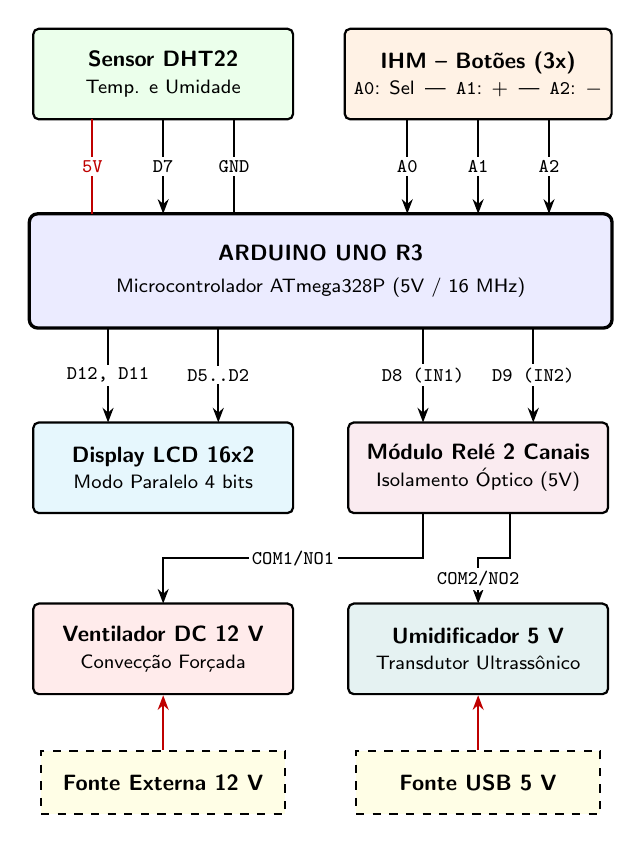
\begin{tikzpicture}[
    font=\footnotesize\sffamily,
    block/.style={draw, rectangle, rounded corners=2pt, thick, minimum width=3.3cm, minimum height=1.15cm, align=center, fill=gray!8},
    arduino/.style={draw, rectangle, rounded corners=3pt, very thick, minimum width=7.4cm, minimum height=1.45cm, align=center, fill=blue!8},
    power/.style={draw, rectangle, dashed, thick, minimum width=3.1cm, minimum height=0.8cm, align=center, fill=yellow!10},
    line/.style={-{Stealth[scale=0.8]}, thick},
    wire/.style={thick},
    pwrline/.style={-{Stealth[scale=0.8]}, thick, red!75!black},
    pwruni/.style={thick, red!75!black},
    lbl/.style={fill=white, inner sep=1.2pt, font=\scriptsize\ttfamily}
]

% Linha 1: Entradas (Sensor DHT22 e Botões IHM)
\node[block, fill=green!8] (dht) at (-2.0, 2.5) {\textbf{Sensor DHT22}\\\scriptsize Temp. e Umidade};
\node[block, fill=orange!10] (btns) at (2.0, 2.5) {\textbf{IHM -- Botões (3x)}\\\scriptsize \texttt{A0}: Sel \,|\, \texttt{A1}: $+$ \,|\, \texttt{A2}: $-$};

% Linha 2: Microcontrolador Central
\node[arduino] (uno) at (0, 0) {\textbf{ARDUINO UNO R3}\\[2pt]\scriptsize Microcontrolador ATmega328P (5V / 16 MHz)};

% Linha 3: Saídas (Display LCD e Módulo Relé)
\node[block, fill=cyan!10] (lcd) at (-2.0, -2.5) {\textbf{Display LCD 16x2}\\\scriptsize Modo Paralelo 4 bits};
\node[block, fill=purple!8] (rele) at (2.0, -2.5) {\textbf{Módulo Relé 2 Canais}\\\scriptsize Isolamento Óptico (5V)};

% Linha 4: Atuadores de Potência
\node[block, fill=red!8] (fan) at (-2.0, -4.8) {\textbf{Ventilador DC 12 V}\\\scriptsize Convecção Forçada};
\node[block, fill=teal!10] (hum) at (2.0, -4.8) {\textbf{Umidificador 5 V}\\\scriptsize Transdutor Ultrassônico};

% Linha 5: Fontes de Alimentação Externas
\node[power] (psu12) at (-2.0, -6.5) {\textbf{Fonte Externa 12 V}};
\node[power] (psu5) at (2.0, -6.5) {\textbf{Fonte USB 5 V}};

% Conexões DHT22 -> Arduino
\draw[pwruni] (-2.9, 1.925) -- node[lbl] {5V} (-2.9, 0.725);
\draw[line]   (-2.0, 1.925) -- node[lbl] {D7} (-2.0, 0.725);
\draw[wire]   (-1.1, 1.925) -- node[lbl] {GND} (-1.1, 0.725);

% Conexões Botões -> Arduino
\draw[line] (1.1, 1.925) -- node[lbl] {A0} (1.1, 0.725);
\draw[line] (2.0, 1.925) -- node[lbl] {A1} (2.0, 0.725);
\draw[line] (2.9, 1.925) -- node[lbl] {A2} (2.9, 0.725);

% Conexões Arduino -> LCD
\draw[line] (-2.7, -0.725) -- node[lbl] {D12, D11} (-2.7, -1.925);
\draw[line] (-1.3, -0.725) -- node[lbl] {D5..D2} (-1.3, -1.925);

% Conexões Arduino -> Relé
\draw[line] (1.3, -0.725) -- node[lbl] {D8 (IN1)} (1.3, -1.925);
\draw[line] (2.7, -0.725) -- node[lbl] {D9 (IN2)} (2.7, -1.925);

% Conexões Relé -> Atuadores
\draw[line] (1.3, -3.075) -- (1.3, -3.65) -- node[lbl] {COM1/NO1} (-2.0, -3.65) -- (-2.0, -4.225);
\draw[line] (2.4, -3.075) -- (2.4, -3.65) -- (2.0, -3.65) -- node[lbl, pos=0.45] {COM2/NO2} (2.0, -4.225);

% Conexões Fontes -> Atuadores
\draw[pwrline] (psu12.north) -- (fan.south);
\draw[pwrline] (psu5.north) -- (hum.south);

\end{tikzpicture}%
}
\caption{Diagrama esquemático de interligação do sistema de climatização em tempo real baseado no Arduino Uno.}
\label{fig:esquematico}
\end{figure}

\subsection{Interface Homem-Máquina e Monitoramento}

Durante a operação contínua, o visor LCD exibe simultaneamente as variáveis ambientais medidas em tempo real (coluna à esquerda) e os valores de referência desejados ou limiares de acionamento (coluna à direita). Na linha superior apresenta-se a temperatura ($T_{\text{atual}} \Rightarrow T_{\text{ref}}$) e, na linha inferior, a umidade relativa do ar ($U_{\text{atual}} \Rightarrow U_{\text{ref}}$).

As tarefas periódicas de aquisição (Tarefas 7 e 8) executaram a leitura do sensor DHT22 e a atualização do visor sem bloquear a resposta aos eventos aperiódicos e esporádicos gerados pelos botões táteis. Por meio dos botões físicos, o usuário pôde alterar dinamicamente os parâmetros $T_{\text{ref}}$ e $U_{\text{ref}}$ em passos discretos de $1{,}00^\circ\text{C}$ e $5{,}00\%$, respectivamente, validando a reconfiguração em tempo de execução prevista na especificação do sistema.

\subsection{Validação Experimental dos Atuadores}

Para verificar a lógica de controle, a exclusão mútua e a resposta física da malha de climatização, conduziram-se ensaios em bancada divididos em três cenários sequenciais de operação, cujos resultados estão sintetizados na Tabela~\ref{tab:resultados_bancada}.

\begin{table}[H]
\centering
\caption{Estados operacionais observados nos testes de bancada do protótipo.}
\label{tab:resultados_bancada}
\scriptsize
\setlength{\tabcolsep}{3pt}
\resizebox{\columnwidth}{!}{%
\begin{tabular}{@{}lcccc@{}}
\toprule
\textbf{Cenário de Teste} & \begin{tabular}[c]{@{}c@{}}\textbf{Temp. ($^\circ$C)}\\$T_{\text{atual}} \Rightarrow T_{\text{ref}}$\end{tabular} & \begin{tabular}[c]{@{}c@{}}\textbf{Umidade (\%)}\\$U_{\text{atual}} \Rightarrow U_{\text{ref}}$\end{tabular} & \textbf{Ventilador} & \textbf{Umidificador} \\ \midrule
1. Repouso Inicial     & $26{,}60 \Rightarrow 30{,}00$ & $72{,}10 \Rightarrow 65{,}00$ & Desligado       & Desligado       \\
2. Limiar Térmico      & $26{,}70 \Rightarrow 24{,}00$ & $71{,}90 \Rightarrow 65{,}00$ & \textbf{Ligado} & Desligado       \\
3. Limiar Higrométrico & $26{,}70 \Rightarrow 24{,}00$ & $71{,}90 \Rightarrow 80{,}00$ & \textbf{Ligado} & \textbf{Ligado} \\ \bottomrule
\end{tabular}%
}
\end{table}

Os comportamentos observados em cada etapa comprovam a aderência do sistema ao modelo projetado:

\begin{itemize}
    \item \textbf{Condição de Conforto (Cenário 1):} Com a temperatura ambiente estabilizada em $26{,}60^\circ\text{C}$ (abaixo do limiar $T_{\text{ref}} = 30{,}00^\circ\text{C}$) e a umidade relativa em $72{,}10\%$ (acima do limiar mínimo $U_{\text{ref}} = 65{,}00\%$), ambos os canais do módulo relé mantiveram-se desenergizados, confirmando a ausência de acionamentos indevidos.
    
    \item \textbf{Atuação Térmica por Convecção (Cenário 2):} Ao reduzir manualmente o limiar $T_{\text{ref}}$ de $30{,}00^\circ\text{C}$ para $24{,}00^\circ\text{C}$, o controlador detectou a condição $T_{\text{atual}} > T_{\text{ref}}$ ($26{,}70^\circ\text{C} > 24{,}00^\circ\text{C}$) e comutou imediatamente o Canal 1 do relé, energizando o ventilador DC de 12~V para promover a circulação de ar e a troca térmica por convecção forçada.
    
    \item \textbf{Atuação Higrométrica e Resposta do Ambiente (Cenário 3):} Mantendo o ventilador ativo, elevou-se o limiar $U_{\text{ref}}$ de $65{,}00\%$ até $80{,}00\%$. Ao ultrapassar a umidade medida ($71{,}90\% < 80{,}00\%$), o Arduino acionou o Canal 2 do relé, alimentando a placa controladora do transdutor piezoelétrico ultrassônico e iniciando a nebulização de água no reservatório. Durante aproximadamente 25~segundos de atuação contínua, o sensor DHT22 registrou a elevação gradual e efetiva da umidade relativa do ambiente de $71{,}90\%$ para $75{,}10\%$, comprovando o acoplamento físico entre a atuação e a variável controlada.
\end{itemize}

\subsection{Análise de Desempenho em Tempo Real}

Sob a ótica de sistemas de tempo real, o escalonamento cíclico não-bloqueante implementado no Arduino Uno (baseado em temporização por hardware via \texttt{millis()}) garantiu que nenhuma tarefa excedesse seu respectivo \textit{deadline} (estabelecidos entre $50~\text{s}$ e $1~\text{min}$). A latência entre o acionamento físico dos botões táteis, a atualização do LCD e a comutação eletromecânica dos relés manteve-se na ordem de dezenas de milissegundos, valor substancialmente inferior às constantes de tempo térmicas e higrométricas do ambiente climatizado. Ademais, o uso de variáveis de estado (\textit{flags}) assegurou a exclusão mútua no acesso aos atuadores, impedindo conflitos lógicos entre comandos manuais e rotinas automáticas.

\begin{thebibliography}{00}
	\bibitem{b1} ASHRAE. Principles of Heating, Ventilating, and Air Conditioning. 10th ed.
	\bibitem{b2} GRAND VIEW RESEARCH. Smart Home Security Market Report. Grand View Research, [2026]. Disponível em: https://www.grandviewresearch.com/industry-analysis/smart-home-security-market-report. Acesso em: 1 out. 2026.
	\bibitem{b3} IMARC GROUP. Brazil Smart Home Market Size, Share, Trends and Forecast by Device Type, Application, Protocol and Region, 2025-2033. IMARC Group, [2026]. Disponível em: https://www.imarcgroup.com/brazil-smart-home-market. Acesso em: 1 out. 2026.
	\bibitem{b4} OGATA, K. Discrete-time control systems. 2nd edition. Englewood Cliffs: Prentice Hall, 1995
	\bibitem{b5} Oliveira, R. S. “Fundamentos dos Sistemas de Tempo Real” 2a Ed.,2020.
	
\end{thebibliography}


\end{document}
